
The study of human-database interaction methods over the past five decades has inspired work in multiple areas including visual query programming, natural language interfaces, speech-driven querying, touch and gesture interaction, and programming by example. 
Even as the database community continues exploring interaction modalities, typing SQL on a keyboard remains the dominant method for database interaction.

The use of SQL programming to query databases aligns with traditional query-result or query-answer paradigms \cite{10.14778/3402755.3402797, 8509430} where database users type and submit a query to a database system and expect a table or scalar result. 
This query-result paradigm places the responsibility to maintain a sufficient level of schema, syntax, and data understanding of the database onto database users.
This involves a certain level of cognitive overhead for effective database interaction. 
The paradigm also requires users to express their intent by employing syntactically and semantically correct SQL statements. 
Although not generally a problem for skilled database practitioners, these knowledge and cognitive requirements can pose as obstacles to new and non-expert database users. 
The desire to improve user experience and remove barriers to extracting knowledge from databases by making database interaction more \emph{natural} to humans continues to motivate research and progress in alternative human-database interaction methods.

Database interaction has been a subject of study for many decades. Some fields of study such as visual query systems have arguable already reached a maturity point, and few opportunities to expand the knowledge base exist to inspire recent research. Natural language interfaces, on the other hand, have benefited from recent rapid advances in machine learning and the advent of transformer-based large language models (LLMs) and have demonstrated significant performance improvements in state of the art systems. 

\subsection{Human Factors and Usability}

The goal of exploring alternative methods of human database interaction is to improve system usability. 
Usability is measurable, and ISO Standard 9241-11 provides criteria for evaluating system usability \cite{10.1007/978-3-319-39510-4_25, 10.1016/S0306-4379(00)00015-6, iso-usability} including measures of effectiveness, efficiency, and satisfaction. 
\textit{Effectiveness} is the measure of a user's ability to complete intended tasks and objectives, the likelihood of errors occuring during task completion, and the intensity or consequence of possible errors. 
\textit{Efficiency} relates to metrics such as the time taken for a user to perform a task, the cost-effectiveness of a system, productive time ratios, the presence (or absence) of unecessary actions, and the amount of fatigue a user may experience when using a system. 
\textit{Satisfaction} is user-focused and based on user studies that collect information relating to overall user satisfaction, user satisfaction with specific features, discretionary (or voluntary) usage of a system or specific features, proportion of users complaining, proportion of complaints about a particular feature, user trust, user pleasure, and physical comfort.

Usability measurements are system-specific and measurement choices in effectiveness, efficiency, and satisfaction are context-driven and determined by the goals of the system and the characteristics of the intended users. 
This system-specific tailoring of usability assessments makes system-vs.-system usability comparisons difficult. 
Several methods have been developed to attempt to standardize these measurements including the \emph{System Usability Scale} (SUS) \cite{sus-retrospective} which is a ten question post-experience questionnaire with alternating (positive and negative) questions and a resulting score ranging from 0 to 100; the \emph{Standardized User Experience Percentile Rank} (SUPR-Q) \cite{suprq}, designed specifically for measuring website quality in terms of user experience; \emph{the Software Usability Meausrement Inventory} (SUMI) \cite{sumi} which is a 50 question questionnaire that scores user experience over multiple criteria including a high-level global score and sub-level scores of efficiency, affect, helpfulness, control, and learnability where scores center around a score of 50 with a standard deviation of 10; the \emph{Usability Metric for User Experience} (UMUX) \cite{10.1016/j.intcom.2010.04.004} which is a very short (4 item) assessment tool with a scoring range from 0 to 40 with outcomes that correlate strongly with the SUS; and the Post-Study System Usability questionnaire (PSSUQ) \cite{pssuq} which is an 18 item questionnaire intended to be administered once a user has completed a system usability study.

\subsubsection{Human Factors in Query Formulation} Siau and Tan describe a framework for query formulation in the user-database interaction process that is based on a three-stage cognitive model of a database query development effort \cite{1637793}:

\begin{enumerate}
  \item Query formulation - form a natural language statement describing data need. (Content)
  \item Query translation - Determine relevant schema elements, query operations, and restrictions to retrieve data need established in prior step. (Constituent Structure)
  \item Query writing - Using a given query language, arrange elements, operations, and restrictions in step 2 into valid syntax. (Style)
\end{enumerate}

% \begin{figure}
%   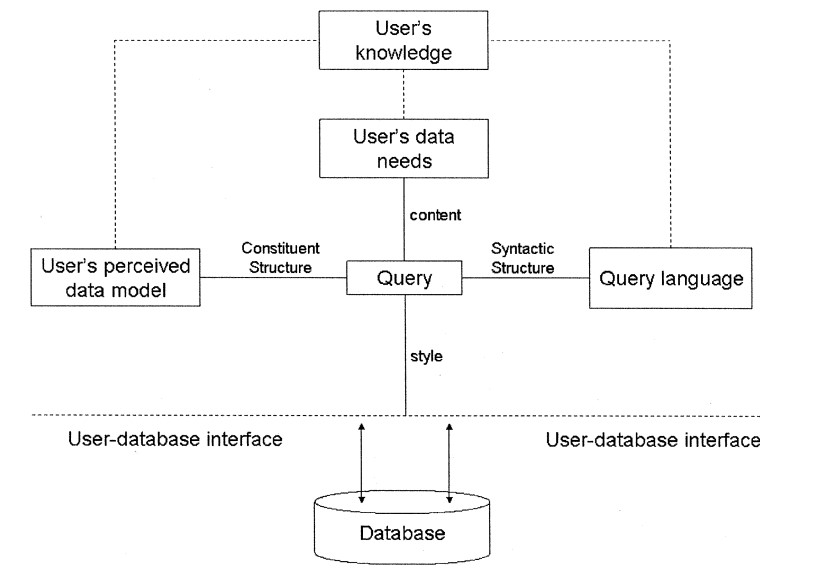
\includegraphics[width=\linewidth]{figures/cognitive_mapping_techniques_for_user_database_interaction_fig_1.jpg}
%   \caption{Sequential Framework for user-database interaction \cite{1637793}}
%   \label{fig:sequential_framework}
% \end{figure}

During this sequential query formulation process, users must contend with human factors-based challenges including cognitive strain, heuristic-driven biases, satisficing, and automaticity, all of which may negatively impact query accuracy and a user's ability to meet their data needs~\cite{1637793}. 
In cases where a query fails to fulfill a user's data needs, an answer understanding and response process may help users make corrections to a faulty query and to steer the query toward their original query intent.

The stepwise approach \cite{10.5555/647248.719775} provides a simplified view of iterative query formulation and modification:

\begin{enumerate}
  \item Understanding - evaluate the schema in the context of a data need and develop a query subschema.
  \item Query formulation - express query operands involved in the intended query using the query subschema developed in the previous step.
  \item Testing - verify that the query expression formed in the prior step fulfills the user's data need.
\end{enumerate}

Interactive frameworks are enabled by the implementation of graphics-based direct manipulation interfaces, conversations with databases using natural language, optimized data sampling and interim result presentation, and other combinations of both familiar and novel techniques.



\subsection{Database Interaction Interfaces}

There are three different levels of database interaction and data model abstraction: physical, logical and conceptual. Abstraction levels represent a transition of power and responsibility between database systems and their users. A high level of abstraction requires users to know less about the underlying physical data configuration and places responsibility on the system to know more about the model as it relates to the world, whereas a lack of abstraction requires users to understand the relationship between the world the data represents and the physical configuration of the data. \cite{10.2307/249587, 1268162} Humans generally interact with databases at the logical and conceptual levels, leaving the database management system to handle the physical-level implementation details.

There are several types of database interaction interfaces including textual (linear keyword or computer language), visual (graphical), and natural language \cite{1637793}. These interfaces generally support a user's interaction with databases during the query formulation, translation, and writing stages. 

\subsubsection{Formal Language}

The most prolific formal database interaction language, and arguably the de-facto industry standard for relational data interaction, is the structured query language (SQL). 
SQL is a relationally complete and declarative language designed to enable interaction with relational data stores at the logical level. 
It was originally designed to improve database accessibility for non-programmers by abstracting away the procedural instructions required to retrieve data from a data store. 
It replaces this process with a declarative language based on relational calculus and relational algebra~\cite{Chamberlin1974}. 
While SQL succeeded in this regard, aspects of its declarative syntax can still present a barrier to entry for those who wish to perform data retrieval and analysis tasks~\cite{10.1145/3514214, 10.1145/2729094.2742620}.

\subsubsection{Natural Language}

Natural language interfaces (NLIs) allow users to interact with databases using unstructured, or semi-structured, language. 
The NLI system takes on the responsibility of translating a user's natural language expression into a formal query that can be executed by the underlying database management system.
The most common contemporary natural language-based interaction method is natural language to SQL (NL-to-SQL), which has been revolutionized by foundational large language models (LLMs)~\cite{openai-chatgpt-blog-post, roziere2023code, anil2023palm}.
With the rapid improvement in natural database interfaces, new challenges emerge that provide opportunities to make the idea of natural interactions with databases a viable and practical technology.


\subsection{Technical Contributions}

\begin{table}[th]
    \centering
    \caption{The types of technical contributions associated with the natural-language interaction projects in this dissertation.}
    \begin{tabular}{p{4cm}p{9cm}}
    \toprule
    \textbf{Project} & \textbf{Contributions} \\
    \midrule
    Chapter 1: SpeakQL 2 & Novel syntax for speech-based querying; Empirical human-computer-interaction-based comparisons and insights\\
    Chapter 2: SNAILS & New benchmark dataset, ML model, LLM prompts; empirical technical comparisons and insights \\
    Chapter 3: SKALPEL & Improved methods; empirical technical comparisons and insights \\
    \bottomrule
    \end{tabular}
    \label{table:contributions}
\end{table}

In this dissertation, we examine 3 areas of natural language database interaction research: speech-based database querying with a natural-like extension of the SQL syntax, schema identifier naming effects on NL-to-SQL performance, and schema reprentations in LLM-based NL-to-SQL pipelines.
The overarching goal of our work in these areas is to improve natural interactions with databases both directly between the user and the database with our SQL syntax extension, and indirectly by improving LLM-based NL-to-SQL translation.
Table~\ref{table:contributions} provides a high-level summary of the contributions in each chapter of this dissertation.
The contributions for each project are as follows:

\paragraph{\textbf{SpeakQL 2: Design and evaluation of an SQL-based dialect for spoken querying}}

In this project, we systematically study and evaluate SpeakQL 2: a syntax extension to SQL tailored for spoken querying.
SpeakQL 2 is an extension of the original SpeakQL project~\cite{Shah2020} that demonstrates the effectiveness of multi-modal speech-based querying.
To further improve speech-based querying, we design the SpeakQL dialect with 4 new features that raise naturalness and reduce syntactic rigidity, while also preserving correct-by-construction guarantees with a context free grammar.
We describe the implementation of the SpeakQL dialect, including its grammar rules and the SpeakQL-to-SQL translation process.

After implementing the SpeakQL syntax in a speech-to-query pipeline, we administer an A/B user study with 23 participants designed to compare the usefulness of SQL and SpeakQL syntax during speech-based querying.
Quantitative analysis of the within-subjects study yielded no statistically significant differences in performance measures including query planning time, number of attempts required to correctly dictate a query, or the number of errors between the 2 dialects.
However, our post-study participant survey surfaces some encouraging pieces of evidence that SpeakQL, despite being a new and slightly more verbose dialect of SQL, takes comparable time to dictate but with a higher ease of use as per the self-reported participant feedback.

As work on the SpeakQL project reached its culmination point, transformer-based large language models and transformer-based automatic speech recognition systems were greatly increasing the accuracy of both NL-to-SQL translation and speech recognition.
This advent largely diminished the value of a more formal syntax designed to guard against inaccurate speech transcriptions and natural language ambiguities, and so the remainder of this dissertation focuses on tackling challenges associated with LLM-based natural language interfaces.

\paragraph{\textbf{SNAILS: Schema naming assessments for improved LLM-based SQL inference}}

With SNAILS, we take the first steps toward a deeper understanding of the effects of schema table and column naming practices on NL-to-SQL performance.
We ask the following 3 interconnected questions: (1) how do we quantify the idea of ``naturalness'' as it relates to the way that schema identifiers are named? (2) Does naturalness impact schema linking accuracy in LLM-based NL-to-SQL and if so, by how much? (3) How much do other factors such as query and database complexity, and language model, impact performance?
To answer these questions, we create a novel integrated benchmark suite we call SNAILS which contains new collections of real-world databases and query pairs, a new labeled dataset of schema identifiers, a set of evaluation metrics, and LLM prompting and other AI artifacts including an ML naturalness classifier.

We find that schema identifier naturalness by and large does have a meaningful effect on NL-to-SQL accuracy and schema linking performance.
Specifically, identifier naturalness is moderately and positively correlated with both schema linking and execution accuracy.
Identifiers of low naturalness yield lower performing NL-to-SQL inferences in terms of both schema linking (identifier recall) and execution accuracy.
These findings have implications for practitioners who are either designing new databases intended for LLM-based applications, or seeking to augment existing RDBMSs with an LLM-based NL-to-SQL interface.

\paragraph{\textbf{SKALPEL: Schema Knowledge Adjustments for LLM NL-to-SQL Performance Enhancements in Large Databases}}

In the SKALPEL paper, we extend the field of recent schema linking research by examining 7 real-world schema subsetting modules reproduced from NL-to-SQL project source code, and testing them over 3 benchmark datasets including Bird, the emergent Spider 2, and schema linking-focused SNAILS--making this the first work to evaluate real-world schema linking modules, using schema linking-focused performance and efficiency metrics, over very large database schemas.
Using the lessons learned from this analysis, we also present a prototype hybrid schema linking method which we call SKALPEL to motivate additional research toward more effective and efficient schema linking.
SKALPEL's specific contributions are: a schema-subsetting specific evaluation framework that isolates schema subsetting modules as an independent process, a reproduction and empirical analysis of 7 real-world schema subsetting moduels from published code repositories, the SKALPEL subsetter prototype designed to improve NL-to-SQL over very large schemas, and the extension of recent schema subsetting research to very large database schemas over newly released NL-to-SQL benchmark datasets.

We find that the overall usefulness of schema subsetting methods is largely dependent on database schema size, with smaller schemas (fewer than 1,000 columns) being susceptible to NL-to-SQL execution accuracy degredation when subsetting is employed.
Conversely, for larger schemas (more than 1,000 columns) LLM-based improvements for open source and smaller economic LLMs benefit from LLM-based subsetting methods, but at the cost of increased token usage.
With these observations, we design a prototype subsetter we call SKALPEL that combines the techniques of natural language question decomposition and semantic search table retrieval that performs as well as LLM-based methods but at a much lower cost in terms of token usage.

\subsection{Summary}